\SourceLeaf{117}
all from the principle that the products of the opposite triangles (those
having only a common vertex or, more concisely, having no common side) into
which the diagonals divide a quadrilateral are equal.

The general barycentric equation among four points, e.\,g. $(A)$, $(B)$, $(C)$,
$(D)$, is
\[
\TriLetter{A}\,(A)+\TriLetter{B}\,(B)+\TriLetter{C}\,(C)+\TriLetter{D}\,(D)=0,
\]
where $\TriLetter{A}$ denotes the triangle $BCD$, $\TriLetter{B}$ the triangle $CDA$,
and so on (with due regard to [the] sign). In our case, if we add to the
preceding notation
\[
\boldsymbol{A}^{*}=\alpha+\gamma+\delta+a+\lambda, \quad \text{etc.}
\]
\[
\boldsymbol{A}^{*}=\omega-\mathfrak{B}-\mathfrak{E}, \quad \text{etc.},
\]
the equation among four points takes the form
\[
\mathfrak{C}(A)+\boldsymbol{D}^{*}(C)=\boldsymbol{A}^{*}(B)+\mathfrak{B}(D),
\]
where $(A)$ denotes the corresponding vertex of the outer pentagon. Equivalently, we have
\[
\begin{gathered}\mathfrak{C}(A)+(\omega-\mathfrak{E}-\mathfrak{C})(C)\\=(\omega-\mathfrak{B}-\mathfrak{E})(B)+\mathfrak{B}(D)\\=(\omega-\mathfrak{E})(e),\end{gathered}
\]
where $(e)$ denotes the corresponding point of the inner pentagon.

\begin{center}\rule{3cm}{.4pt}\end{center}

\begin{center}\resizebox{7cm}{!}{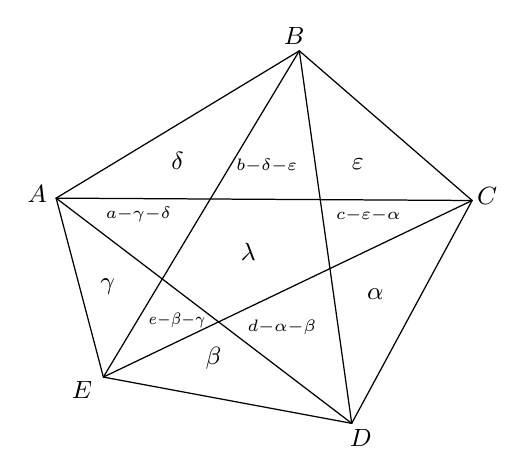
\begin{tikzpicture}[x=.006cm,y=-.006cm,line width=.45pt,line cap=round,line join=round,every node/.style={inner sep=0pt,font=\small}]
\coordinate (A) at (158,408);
\coordinate (B) at (673,96);
\coordinate (C) at (1039,413);
\coordinate (D) at (784,885);
\coordinate (E) at (258,787);
\draw (A) -- (B);
\draw (B) -- (C);
\draw (C) -- (D);
\draw (D) -- (E);
\draw (E) -- (A);
\draw (A) -- (C);
\draw (A) -- (D);
\draw (B) -- (E);
\draw (B) -- (D);
\draw (C) -- (E);
\node at (118,400) {$A$};
\node at (662,65) {$B$};
\node at (1071,403) {$C$};
\node at (803,916) {$D$};
\node at (213,814) {$E$};
\node at (415,330) {$\delta$};
\node at (604,339) {$\scriptstyle b-\delta-\varepsilon$};
\node at (797,337) {$\varepsilon$};
\node at (332,443) {$\scriptstyle a-\gamma-\delta$};
\node at (819,445) {$\scriptstyle c-\varepsilon-\alpha$};
\node at (565,522) {$\lambda$};
\node at (267,596) {$\gamma$};
\node at (414,666) {\scalebox{.86}[1]{$\scriptstyle e-\beta-\gamma$}};
\node at (491,747) {$\beta$};
\node at (636,681) {$\scriptstyle d-\alpha-\beta$};
\node at (834,612) {$\alpha$};
\end{tikzpicture}
}\end{center}

\[
\boldsymbol{A}c\varepsilon+\boldsymbol{C}c(b-\varepsilon)=\boldsymbol{B}b(c-\varepsilon)+\boldsymbol{D}b\varepsilon,
\]
\[
\boldsymbol{B}d\alpha+\boldsymbol{D}d(c-\alpha)=\boldsymbol{C}c(d-\alpha)+\boldsymbol{E}c\alpha,
\]
\[
\boldsymbol{C}e\beta+\boldsymbol{E}e(d-\beta)=\boldsymbol{D}d(e-\beta)+\boldsymbol{A}d\beta,
\]
\[
\boldsymbol{D}a\gamma+\boldsymbol{A}a(e-\gamma)=\boldsymbol{E}e(a-\gamma)+\boldsymbol{B}e\gamma,
\]
\[
\boldsymbol{E}b\delta+\boldsymbol{B}b(a-\delta)=\boldsymbol{A}a(b-\delta)+\boldsymbol{C}a\delta,
\]
